\documentclass{article}
\usepackage[utf8]{inputenc}
\usepackage{amsmath}
\usepackage{amssymb}
\usepackage{graphicx}

\newcommand\xk{\mathbf{x}^{\left(k\right)}}
\newcommand\xkn{\mathbf{x}^{\left(k+1\right)}}
\newcommand\yk{\mathbf{y}^{\left(k\right)}}
\newcommand\ykn{\mathbf{y}^{\left(k+1\right)}}

\newcommand\xn{\mathbf{x}^{\left(0\right)}}
\newcommand\yn{\mathbf{y}^{\left(0\right)}}

\newcommand\xo{\mathbf{x}^{\left(1\right)}}
\newcommand\yo{\mathbf{y}^{\left(1\right)}}


\begin{document}

\section*{Modified Newton method}
For the solution of the non-linear system of equations$\mathbf{F}\left(\mathbf{x}\right) = \textbf{0}$ (with $\mathbf{F}:\mathbb{R}^{n} \to \mathbb{R}^{n}$), the following iterative method has been proposed:
\begin{align}
    \yk &= \xk + \mathrm{D}\mathbf{F}\left(\xk\right)^{-1} \mathbf{F}\left(\xk\right) \\
    \xkn &= \yk - \mathrm{D}\mathbf{F}\left(\xk\right)^{-1} \mathbf{F}\left(\yk\right)
\end{align}
where $\mathrm{D}\mathbf{F}\left(\mathbf{x}\right) \in \mathbb{R}^{n,n}$ is the Jacobian matrix of $\mathbf{F}$ evaluated in the point $\mathbf{x}$.

\subsection*{8-9.a}
We should assume for this subtask that $\mathbf{F}$ is \textbf{injective}, hence for any $\mathbf{x}, \mathbf{y} \in \mathbb{R}^{n}$ we have $\mathbf{F}\left(\mathbf{x}\right) = \mathbf{F}\left(\mathbf{y}\right) \implies \mathbf{x} = \mathbf{y}$. We need to show that under this assumption the iteration given by (1) and (2) is \textbf{consistent} with $\mathbf{F}\left(\mathbf{x}\right) = \mathbf{0}$.

\begin{figure}[!hbt]
    \centering
    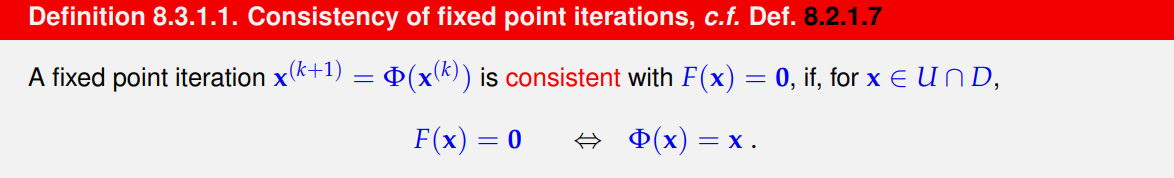
\includegraphics[width=1.1\linewidth]{ConsistendyDef.png}
\end{figure}
\noindent Here the expression $\Phi\left(\mathbf{x}\right) = \mathbf{x}$ can be rewritten to $\xk = \mathbf{x}^{\left(0\right)}$ for every $k \in \mathbb{N}$ for a fixed point of the iteration. Let us assume that we are given a fixed point $\mathbf{x}^{*}$ for the iteration and that $\mathrm{D}\mathbf{F}\left(\mathbf{x}^{*}\right)$ is regular. We will prove both statements of the if and only if statement.
\paragraph{$\mathbf{F}\left(\mathbf{x}^{\left(0\right)}\right) = \mathbf{0} \implies \xk = \mathbf{x}^{\left(0\right)} \: \forall\, k \in \mathbb{N}$:} Let us hence assume that $\mathbf{F}\left(\mathbf{x}^{\left(0\right)}\right) = \mathbf{0}$ is true, evaluating the iterative step given by (1) and (2):
\begin{align*}
    \yn &= \xn + \mathrm{D}\mathbf{F}\left(\xn\right)^{-1} \mathbf{0} = \xn \\
    \xo &= \xn - \mathrm{D}\mathbf{F}\left(\xn\right)^{-1} \mathbf{F}\left(\xn\right) = \xn - \mathrm{D}\mathbf{F}\left(\xn\right)^{-1} \mathbf{0} = \xn 
\end{align*}
We hence can produce an inductive proof. The base case was just proven, assuming the claim holds for some $k \in \mathbb{N}$ we can do the following induction step 
\begin{align*}
    \yk &= \xk + \mathrm{D}\mathbf{F}\left(\xk\right)^{-1} \mathbf{0} = \xk \\
    \xkn &= \xk - \mathrm{D}\mathbf{F}\left(\xk\right)^{-1} \mathbf{F}\left(\xk\right) = \xk - \mathrm{D}\mathbf{F}\left(\xk\right)^{-1} \mathbf{0} = \xk 
\end{align*}
and can conclude that the statement holds for any $k \in \mathbb{N}$. This concludes the proof for this direction.

\pagebreak

\paragraph{$\mathbf{F}\left(\mathbf{x}^{\left(0\right)}\right) = \mathbf{0} \impliedby\xk = \mathbf{x}^{\left(0\right)} \: \forall\, k \in \mathbb{N}$:} Let us assume that  $\xk = \mathbf{x}^{\left(0\right)}$ is true for all$k \in \mathbb{N}$. Let us look at the iteration step
\begin{align*}
    \yk &= \xk + \mathrm{D}\mathbf{F}\left(\xk\right)^{-1} \mathbf{F}\left(\xk\right) \\
    \xkn &= \yk - \mathrm{D}\mathbf{F}\left(\xk\right)^{-1} \mathbf{F}\left(\yk\right)
\end{align*}
Which because of our assumption can be rewritten as
\begin{align*}
    \yk &= \xk + \mathrm{D}\mathbf{F}\left(\xk\right)^{-1} \mathbf{F}\left(\xk\right) \\
    \xk &= \yk - \mathrm{D}\mathbf{F}\left(\xk\right)^{-1} \mathbf{F}\left(\yk\right)
\end{align*}
Hence we can put the first equation into the second one and get
\begin{equation*}
    \xk = \xk + \mathrm{D}\mathbf{F}\left(\xk\right)^{-1} \mathbf{F}\left(\xk\right) - \mathrm{D}\mathbf{F}\left(\xk\right)^{-1} \mathbf{F}\left(\xk + \mathrm{D}\mathbf{F}\left(\xk\right)^{-1} \mathbf{F}\left(\xk\right)\right)
\end{equation*}
We subtract $\xk$ on both sides and get
\begin{equation*}
    \mathbf{0} = \mathrm{D}\mathbf{F}\left(\xk\right)^{-1} \mathbf{F}\left(\xk\right) - \mathrm{D}\mathbf{F}\left(\xk\right)^{-1} \mathbf{F}\left(\xk + \mathrm{D}\mathbf{F}\left(\xk\right)^{-1} \mathbf{F}\left(\xk\right)\right)
\end{equation*}
We then multiply both sides with $\mathrm{D}\mathbf{F}\left(\xk\right)$ from the left (remember that $\mathrm{D}\mathbf{F}\left(\xk\right)$ is regular and thus invertible).
\begin{equation*}
    \mathbf{0} = \mathbf{F}\left(\xk\right) - \mathbf{F}\left(\xk + \mathrm{D}\mathbf{F}\left(\xk\right)^{-1} \mathbf{F}\left(\xk\right)\right)
\end{equation*}
Using the injectivity of $\mathbf{F}$ we get that
\begin{equation*}
    \mathbf{0} = \mathbf{F}\left(\xk\right) - \mathbf{F}\left(\xk + \mathrm{D}\mathbf{F}\left(\xk\right)^{-1} \mathbf{F}\left(\xk\right)\right) \implies \mathrm{D}\mathbf{F}\left(\xk\right)^{-1} \mathbf{F}\left(\xk\right) = \mathbf{0}
\end{equation*}
Again multiplying both sides from the left with $\mathrm{D}\mathbf{F}\left(\xk\right)$ gives us 
\begin{equation*}
     \mathbf{F}\left(\xk\right) = \mathbf{0}
\end{equation*}
which concludes the proof of this side. As we have proven both implications we can conclude that the iteration is \textbf{consistent} with $\mathbf{F}\left(\mathbf{x}\right) = \mathbf{0}$.

\pagebreak

\subsection*{8-9.b} For a scalar method $F$, i.e. n = 1, the iterative method reduces to
\begin{align*}
    \yk &= \xk + \mathbf{F}'\left(\xk\right)^{-1}\mathbf{F}\left(\xk\right) \\
    \xkn &= \yk - \mathbf{F}'\left(\xk\right)^{-1}\mathbf{F}\left(\yk\right)
\end{align*}
We are given the function $f$ and its derivative $\mathrm{d}f$, how do we get the inverse? This is not needed here, because in the case of $n = 1$ we have that 
\begin{equation*}
    \text{If } n = 1\text{ then } \mathbf{F}'\left(\xk\right)^{-1} = \frac{1}{\mathbf{F}'\left(\xk\right)}
\end{equation*}
Hence we can just divide by the value the derivative produces. This produces the following code.

\begin{figure}[!hbt]
    \centering
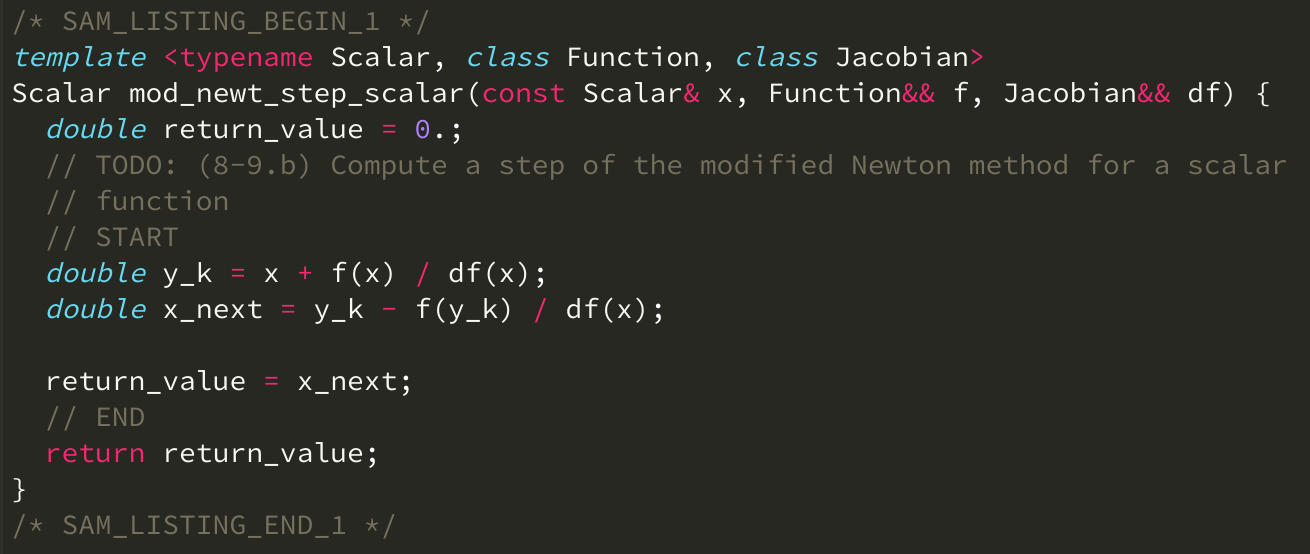
\includegraphics[width=1.0\linewidth]{8-9.b.png}
\end{figure}
\subsection*{8-9.c}
We are now tasked with determining the order of convergence of the newton iteration implemented in 8-9.b using the following function
\begin{equation*}
    \arctan\left(x\right) - 0.123 = 0
\end{equation*}
For this we should use the following fraction to determine empirically the order of convergence (assuming $p > 1$)
\begin{equation}
   \text{For } \epsilon_{k} := \left\lVert \xk -\mathbf{x}^{*}\right\rVert \text{ we have } p \approx \frac{\log\left(\epsilon_{k+1}\right)-\log\left(\epsilon_{k}\right)}{\log\left(\epsilon_{k}\right) - \log\left(\epsilon_{k-1}\right)}
\end{equation}
and we should also implement a meaningful stopping criterion. We will do this first. Looking at the function declaration we can see that we are given only one error tolerance, which indicates that we could use correction based termination in combination with a maximum number of iteration, this was determined again by looking at the function declaration which comes with a \textit{max\_itr} parameter. We use the following termination criterion

\begin{equation*}
    \epsilon_{k} < \tau \left\lVert \xk\right\rVert
\end{equation*}
In the code the variable \textit{eps} is $\tau$, which of course was chosen in a way to ensure maximal ambiguity and confusion. In a next step we will have to implement the method \textit{sample\_nonlinear\_solver} which performs many steps of the Newton-Iteration and determines the order of convergence. We will have to supply it with all the necessary functions from a method call in \textit{mod\_newt\_ord}. This gives us the following code.

\begin{figure}[!hbt]
    \centering
    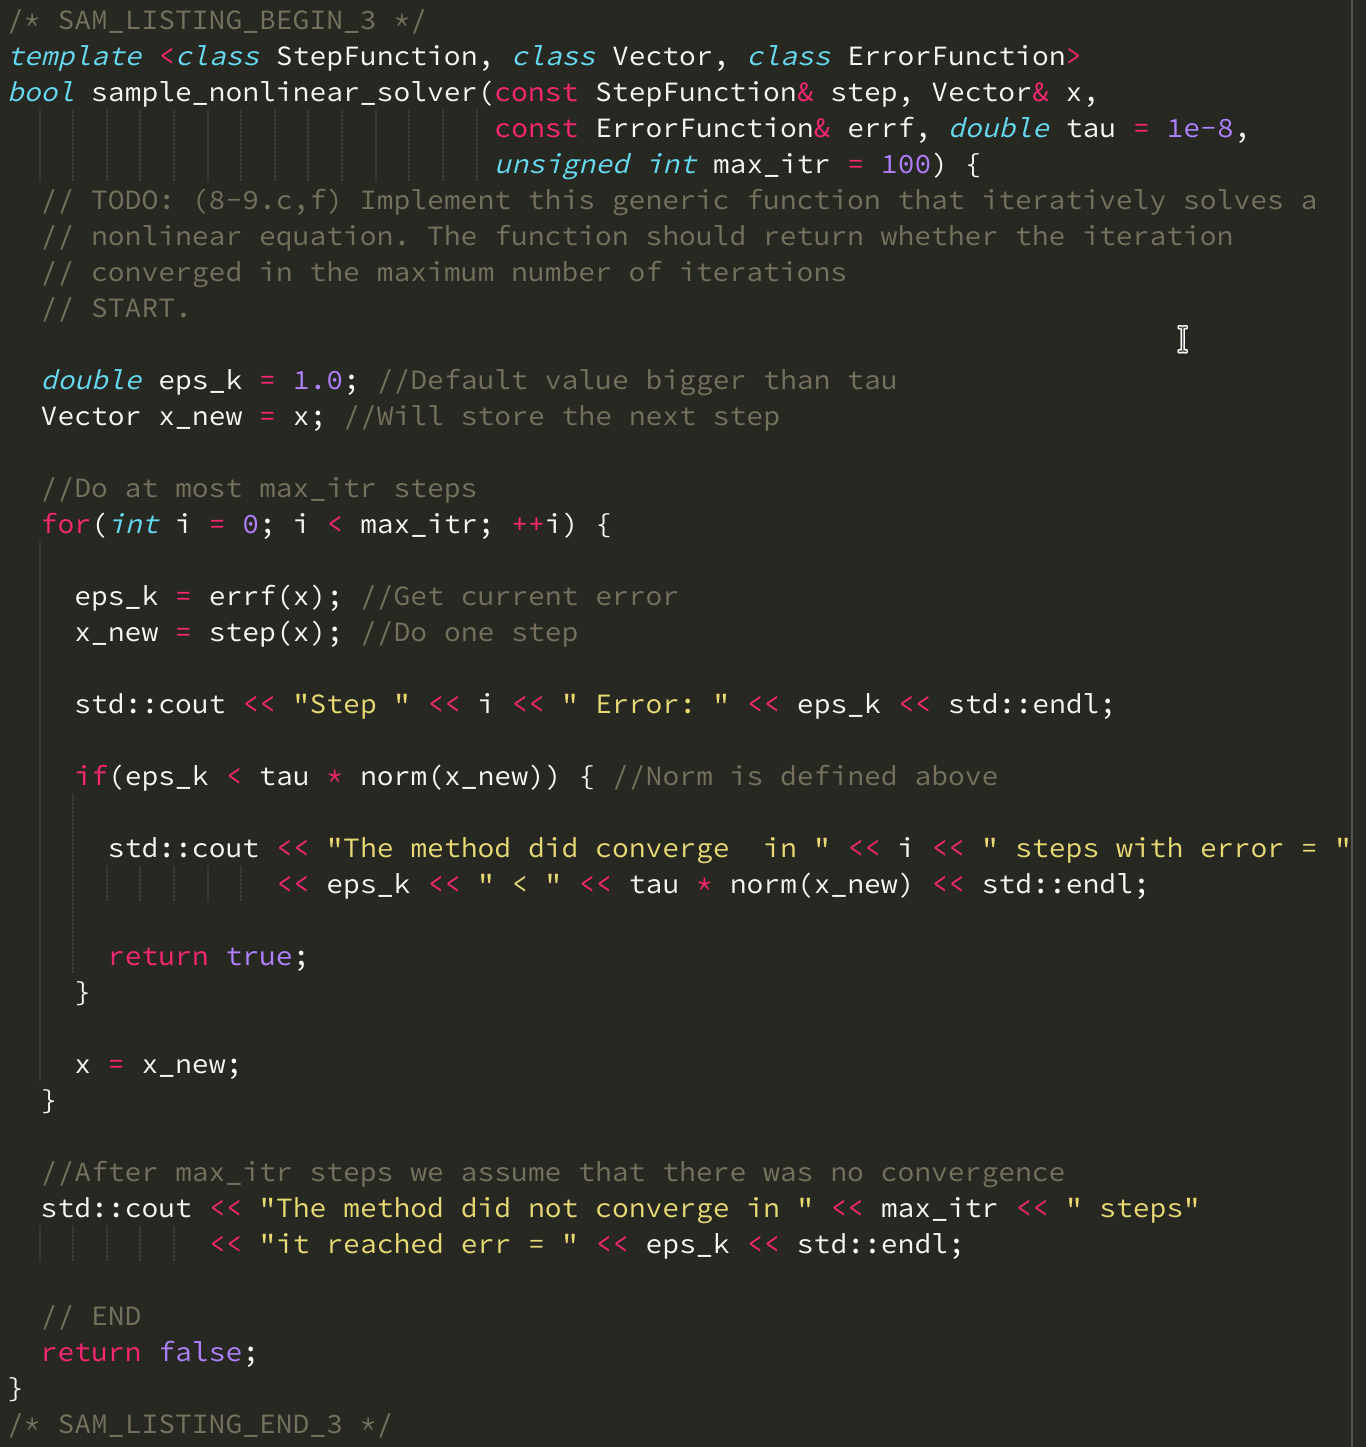
\includegraphics[width=0.8\linewidth]{8-9.c.png}
\end{figure}
Now for the implementation of the methods that are used to call this method. We have the step function that is already implemented, we need to make a functor from it. Also beware that Vector stand for std::vector here. The derivative of $\mathbf{F}\left(x\right) = \arctan\left(x\right) -0.123$ is
\begin{equation*}
    \mathbf{F}'\left(x\right) = \frac{1}{1+x^{2}}
\end{equation*}
Finally the error is given to us by
\begin{equation*}
    \text{error } = \left\lVert \xk - \mathbf{x}^{*}\right\rVert
\end{equation*}
Where we have 
\begin{equation*}
    \mathbf{x}^{*} = \tan\left(0.123\right) = 0.123624065869274\dots
\end{equation*}
We will now implement this in code. It is also important to see that we store each result in Vectors which is achieved via calling the functors. This results in the following code.
\begin{figure}[!hbt]
    \centering
    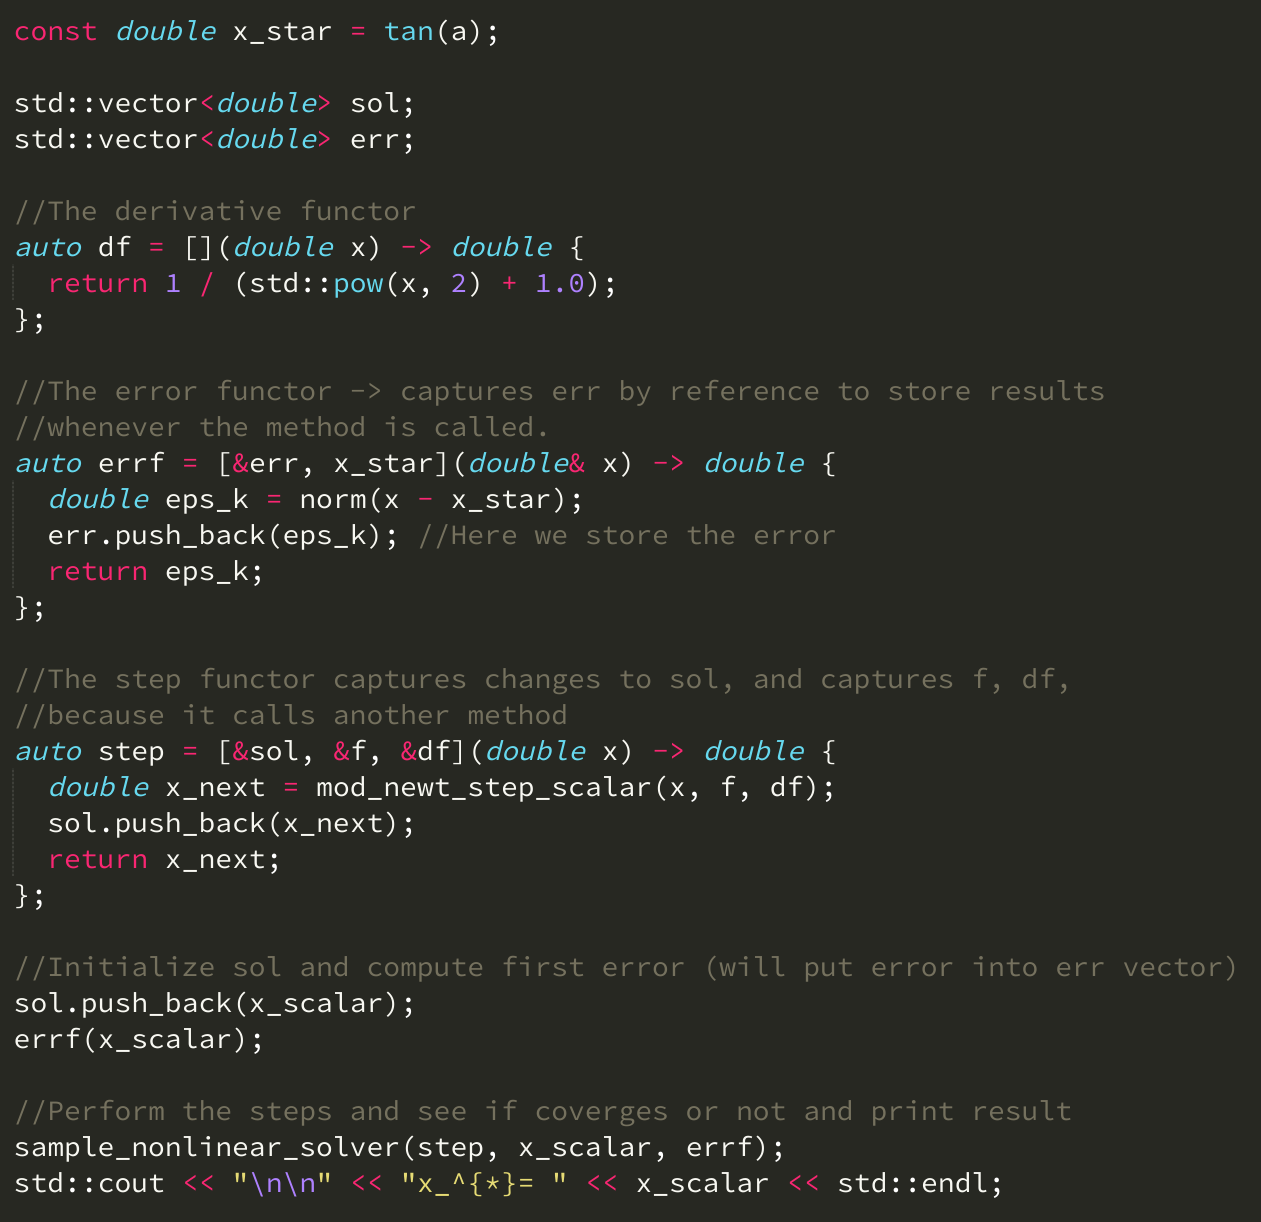
\includegraphics[width=0.9\linewidth]{8-9.c2.png}
\end{figure}

For the actual error computation we use the computed results and then (3) to get the convergence order. 

\pagebreak

We again implement a functor for the convergence term. This gives us the following code.

\begin{figure}[!hbt]
    \centering
    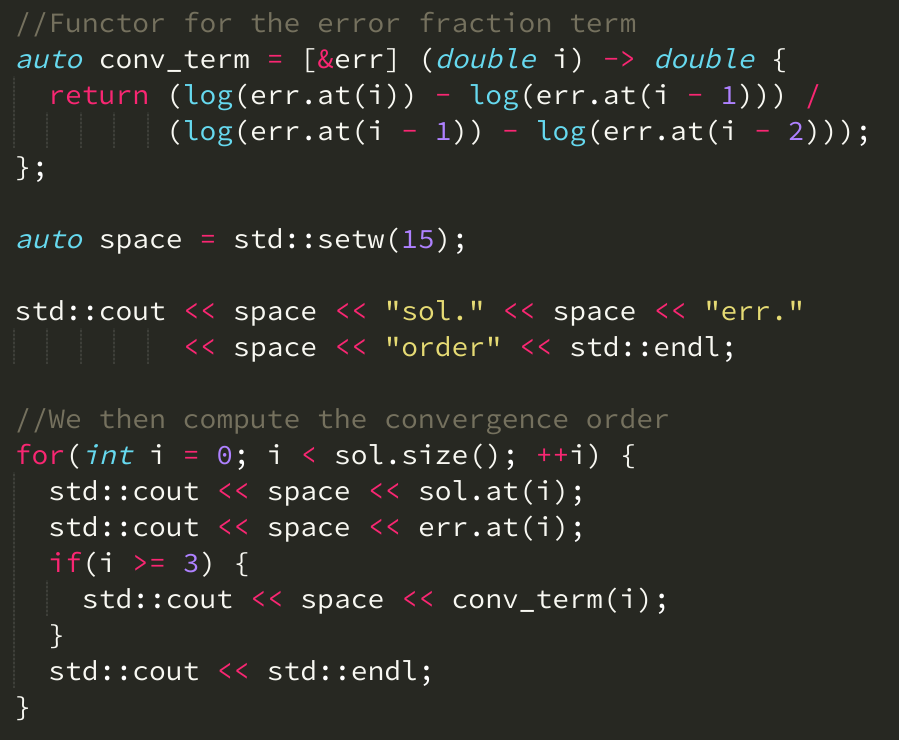
\includegraphics[width=0.9\linewidth]{8-9.c3.png}
\end{figure}
From the data we can say that the order is between $2$ and $3$.
\subsection*{8-9.d} 
In this subtask we are tasked with implementing the modified Newton iteration as given in (1) and (2).
\begin{align}
    \yk &= \xk + \mathrm{D}\mathbf{F}\left(\xk\right)^{-1} \mathbf{F}\left(\xk\right) \\
    \xkn &= \yk - \mathrm{D}\mathbf{F}\left(\xk\right)^{-1} \mathbf{F}\left(\yk\right)
\end{align}
We are given as parameters the point $x$, the function $f$ and the Jacobian as $df$. The sentence " whereas the type Jacobian must have
an evaluation operator that returns an object compatible with Eigen::MatrixXd." tells us that we can apply Eigen operations to the Jacobian, this is how we will get the inverse. We can use the LU-decomposition of the Jacobian to get the term
\begin{equation*}
\mathrm{D}\mathbf{F}\left(\xk\right)^{-1} \mathbf{F}\left(\xk\right)
\end{equation*}
By solving 
\begin{equation*}
       \mathrm{D}\mathbf{F}\left(\xk\right)\mathbf{v} = \mathbf{F}\left(\xk\right)
\end{equation*}
Where $\mathbf{v}$ is some meaningless placeholder variable to avoid confusion. We also compute using the same LU-decomposition 
\begin{equation*}
    \mathrm{D}\mathbf{F}\left(\xk\right)^{-1} \mathbf{F}\left(\yk\right)
\end{equation*}
by solving 
\begin{equation*}
       \mathrm{D}\mathbf{F}\left(\xk\right)\mathbf{w} = \mathbf{F}\left(\yk\right)
\end{equation*}
This produces the following code
\begin{figure}[!hbt]
    \centering
    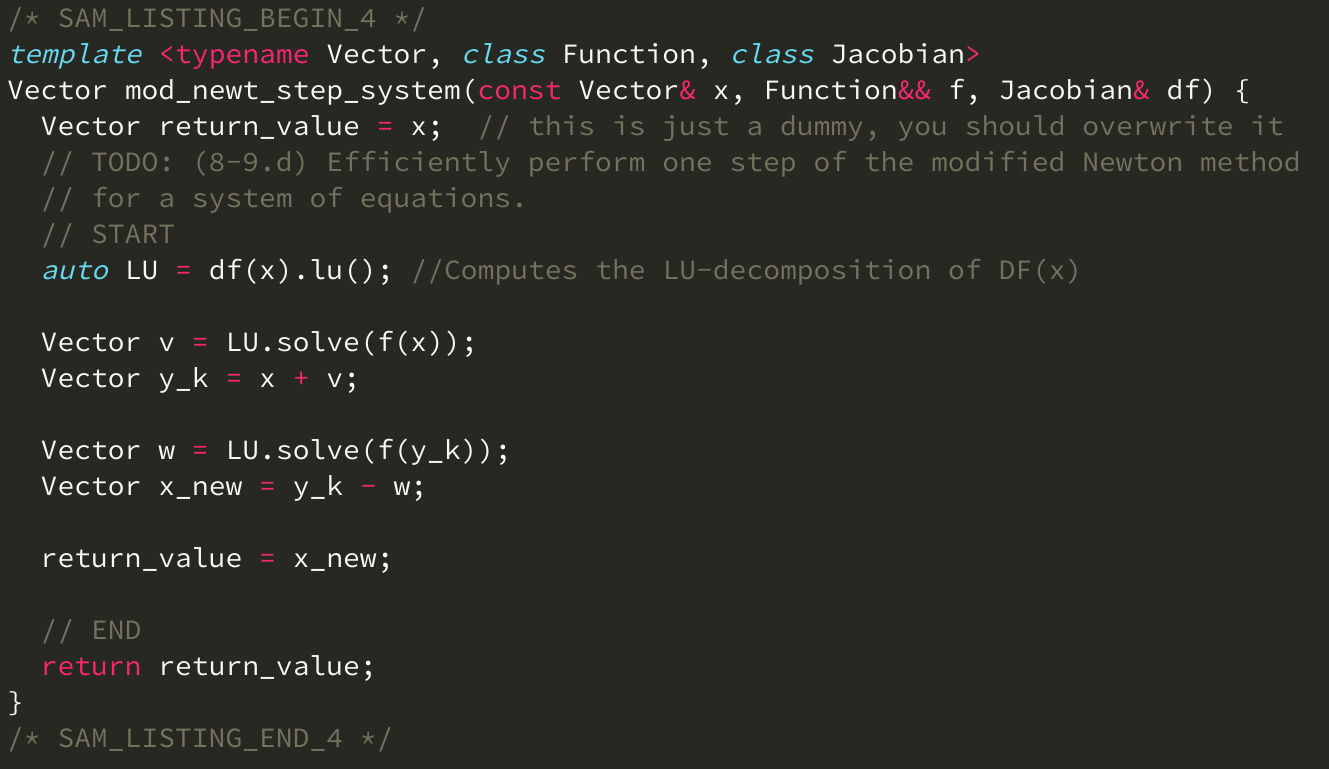
\includegraphics[width=1.0\linewidth]{8-9.c4.png}
\end{figure}
\subsection*{8-9.d} We now conside the following non-linear system of equations
\begin{equation*}
    \mathbf{F}\left(\mathbf{x}\right) := \mathbf{A}\mathbf{x} + \begin{bmatrix}
        c_{1}e^{x_{1}} \\
        \vdots 
        \\
        c_{n}e^{x_{n}} 
    \end{bmatrix}= \mathbf{0}
\end{equation*}
$\mathbf{A}\in \mathbb{R}^{n,n}$ is symmetric positive definite and for all $i = 1, \dots, n $ we have $c_{i} \geq 0$. We should now compute the Jacobi-Matrix of $\mathbf{F}$. We can use that we can treat each of the terms separately.
\begin{equation*}
    \mathrm{D}\mathbf{F}\left(\mathbf{x}\right) := \mathrm{D}\mathbf{A}\mathbf{x} + \mathrm{D}\begin{bmatrix}
        c_{1}e^{x_{1}} \\
        \vdots 
        \\
        c_{n}e^{x_{n}} 
    \end{bmatrix} = \mathbf{A} + \begin{bmatrix}
        c_{1}e^{x_{1}} & 0 & \dots && & \dots & 0 \\
        0 & c_{2}e^{x_{2}} & 0& \dots && \dots & 0 \\
        \vdots & \vdots & \ddots & & & & 0 \\
        \\
        \vdots & \vdots &  & & &\ddots & \vdots \\
        0 & 0 &&&& \dots & c_{n}e^{x_{n}}
    \end{bmatrix}
\end{equation*}
\subsection*{8-9.f} 
We are now tasked to solve $\mathbf{F}\left(\mathbf{x}\right)$ as defined above. The matrix $\mathbf{A}$ is passed as argument, and we also are given a tolerance argument and a maximum iteration limit as arguments. As a hint we are told that we could use the \textit{sample\_nonlinear\_solver} method which we already implemented. For this to work we would have to implement the step and the error function as functors, furthermore the step requires the derivate as functor as well, hence we will implement these first. The following code should work in theory, but there is an error, if I find out why I will edit this file.
\begin{figure}[!hbt]
    \centering
    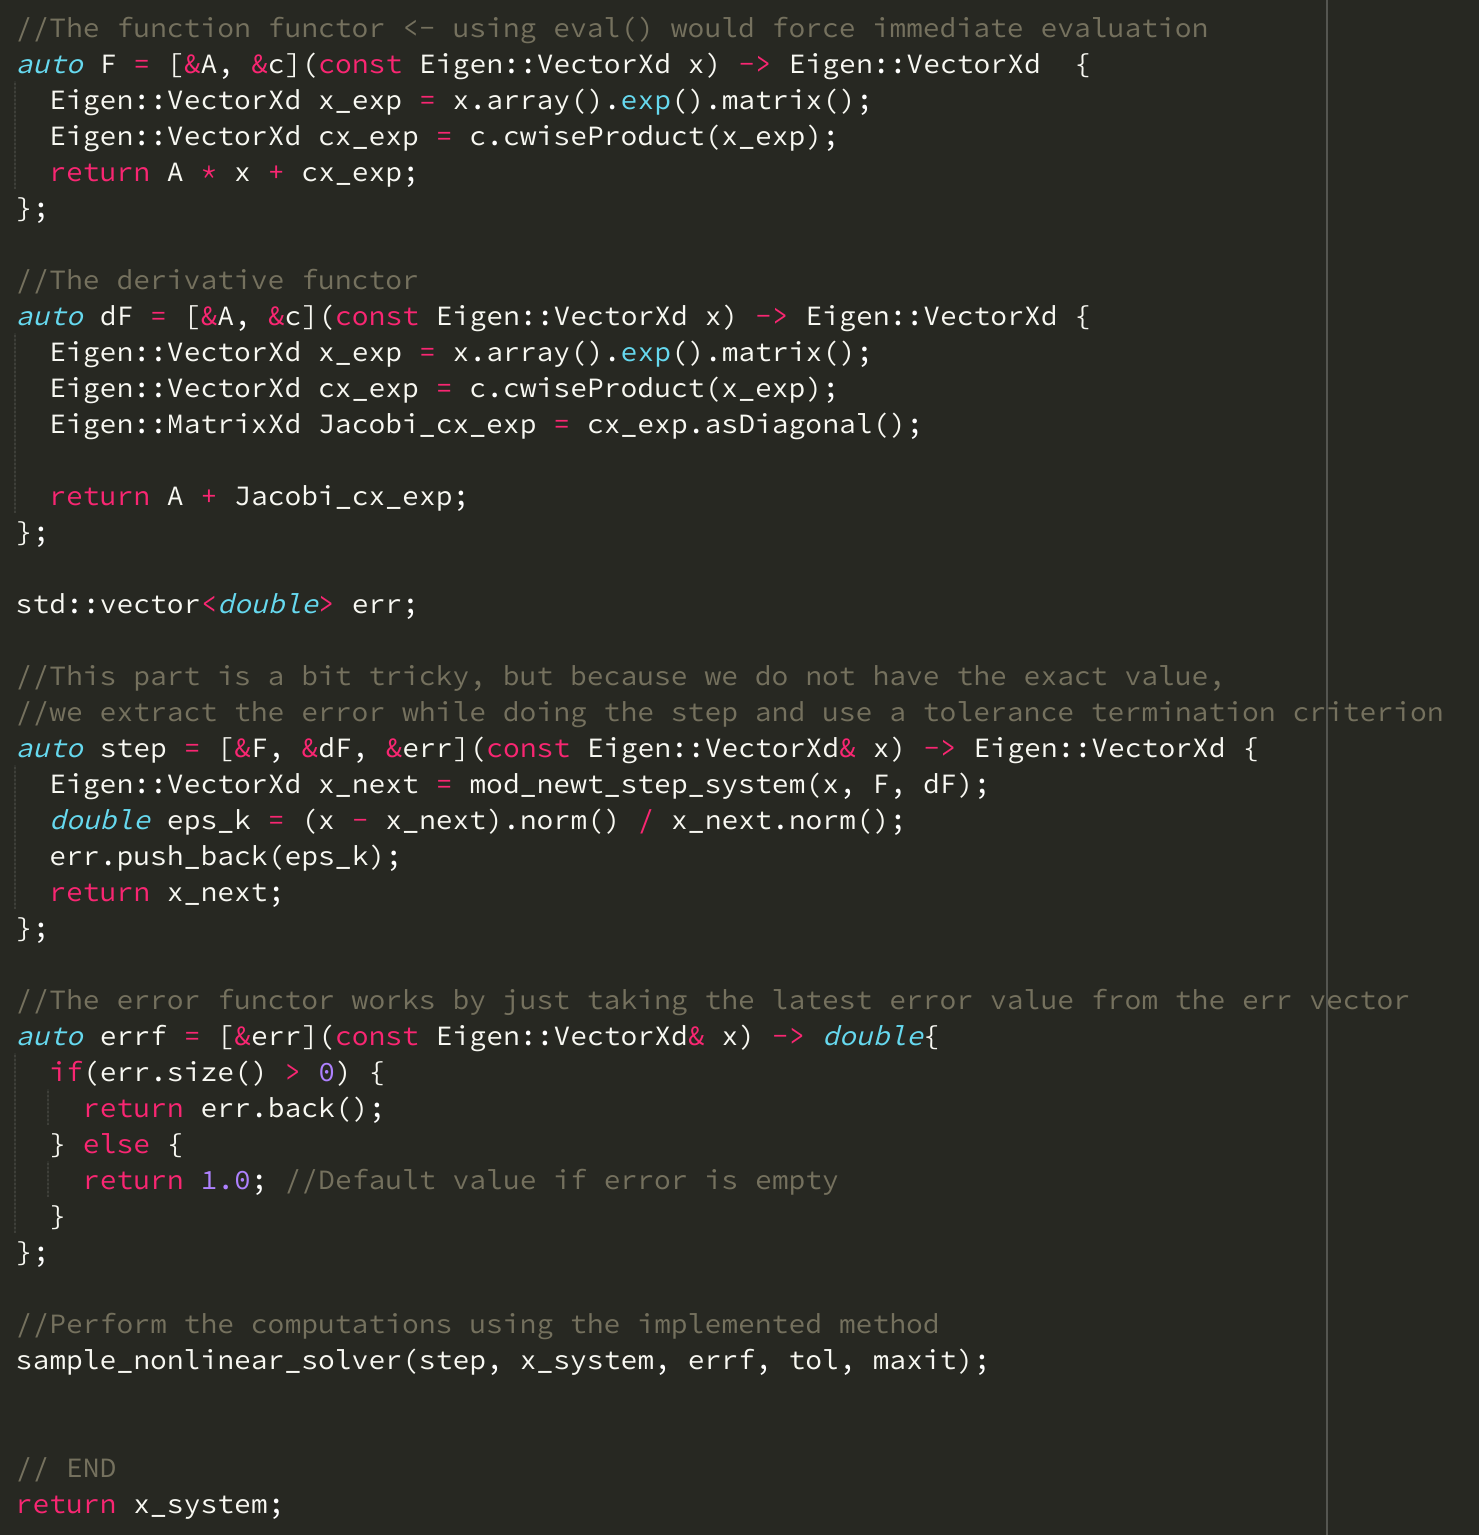
\includegraphics[width=1.0\linewidth]{8-9.c5.png}
\end{figure}

I found the mistake it was that the derivative functor returned a vector instead of a matrix, and a vector is not a dynamic type in all dimensions (has one column exactly), hence the LU solver has a problem with it. This fixes the problem.

\begin{figure}[!hbt]
    \centering
    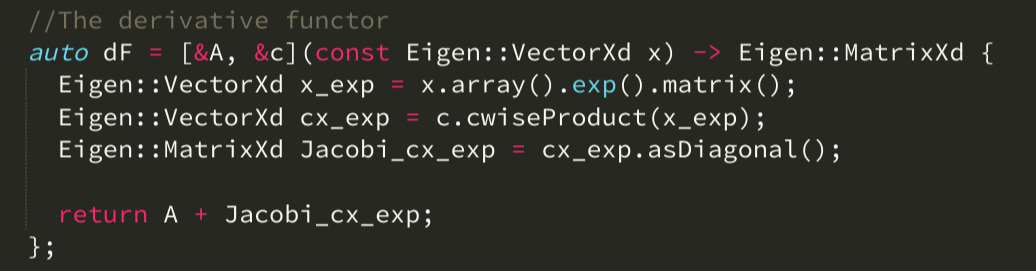
\includegraphics[width=1.0\linewidth]{MistakeCorrected.png}
\end{figure}

Here is the corrected version. 

\subsection*{8-9.g} 
This task is almost the same as a previous one and little to no learning could be achieved here,for this reason I skipped this.
\end{document}
